\documentclass[10pt]{article}

% Pacotes extras necessários
\usepackage{amsmath}
\usepackage[lmargin=0.5in, rmargin=0.5in, tmargin=0.5in, bmargin=0.5in, includehead, includefoot]{geometry}
\usepackage{amsfonts}
\usepackage[utf8]{inputenc}
\usepackage[portuguese]{babel}
\usepackage{graphicx}
\usepackage{fancyhdr}
\usepackage{setspace}

\graphicspath{ {./images/} }

% Sets para outras partes
\setlength{\parindent}{0pt}
\setstretch{1.5}
\DeclareMathOperator{\sen}{sen}
\DeclareMathOperator{\sinc}{sinc}

%% Facilidades
%% -- Laplace
\newcommand{\Lap}[1]{\mathcal{L}\left\{#1\right\}}

%% -- Negrito em matemáticas
\newcommand{\bm}[1]{\boldsymbol{#1}}


% ------- Estilo do trabalho -------- %
\fancypagestyle{capa}{
    \fancyhf{}
    \renewcommand\headrulewidth{0pt}
    \fancyfoot[C]{
        Rio de Janeiro\\
        2023
    }
}

\pagestyle{fancy}
\fancyhead{}
\fancyhead[L]{\thepage}
\fancyfoot{}
% ----------------------------------- %

% Dados do Grupo
\title{Modelagem de Sistemas Dinâmicos - Trabalho Nº1}
\author{
    Leonardo Soares da Costa Tanaka - DRE: 121067652
}
\date{}

\begin{document}
\maketitle
\thispagestyle{capa}
\newpage

Considerando um sistema linear invariante no tempo de u(t), saída y(t) e 
função de transferência dada por:

\begin{align*}
    H(s) = \frac{100}{16} \frac{s^2 + 16}{s^2 + 0.2s + 100}
\end{align*}

Escrevendo $H(jw)$:

\begin{align*}
    H(jw) = H(s)|_{s=jw} = \frac{100}{16} \frac{(jw)^2 + 16}{(jw)^2 + 0.2jw + 100} = \frac{100}{16} \frac{16 - w^2}{0.2jw + 100 - w^2}
\end{align*}

Calculando o módulo da função de trasnferência:

\begin{align*}
    |H(jw)| = \frac{100}{16} \frac{\sqrt{(16 - w^2)^2}}{\sqrt{(0.2)^2 + (100 - w^2)^2}}
\end{align*}

Calculando a fase da função de transferência:

\begin{align*}
    \angle H(jw) = arctan(0/(16 - w^2)) - arctan(0.2w/(100 - w^2))
\end{align*}

1. Foi considerado uma entrada $u(t) = cos(t) 1(t)$. Foi obtido a $y(t)$ por simulação numérica utilizando Python
e as bibliotecas NumPy, Matplotlib e Control.

\begin{verbatim}
    import numpy as np
    import control as ctrl
    import matplotlib.pyplot as plt
    
    # 1. Definir a função de transferência do sistema
    num = [100, 0, 1600]  # numerador da função de transferência
    den = [16, 3.2, 1600]  # denominador da função de transferência
    sys = ctrl.TransferFunction(num, den)  # criar o objeto que representa o sistema
    
    # 2. Definir os valores de tempo para simulação
    t = np.linspace(0, 4*np.pi, 10000)  # valores de tempo de 0 a 2*pi segundos
    
    # 3. Definir o sinal de entrada como o cosseno multiplicado pelo degrau unitário
    u = np.heaviside(t, 1) * np.cos(t)
    
    # 4. Realizar a simulação da resposta do sistema usando a função `control.forced_response()`
    t_out, yout= ctrl.forced_response(sys, T=t, U=u)
    
    # 5. Calcular a frequência da resposta
    Y = np.fft.fft(yout)
    mag = np.abs(Y)
    idx = np.argmax(mag)
    freq = np.fft.fftfreq(len(t), t[1]-t[0])[idx]
    print('A frequência da resposta é:', freq, 'rad/s')
    
    # 6. Plotar o gráfico da resposta
    plt.plot(t_out, yout)
    plt.xlabel('t')
    plt.ylabel('y(t)')
    plt.title('Resposta ao cosseno multiplicado pelo degrau unitário')
    plt.show()    
\end{verbatim}

Resultado obtido foi: A frequência da resposta é: -1.5913902759758614 rad/s

\begin{figure}[h]
    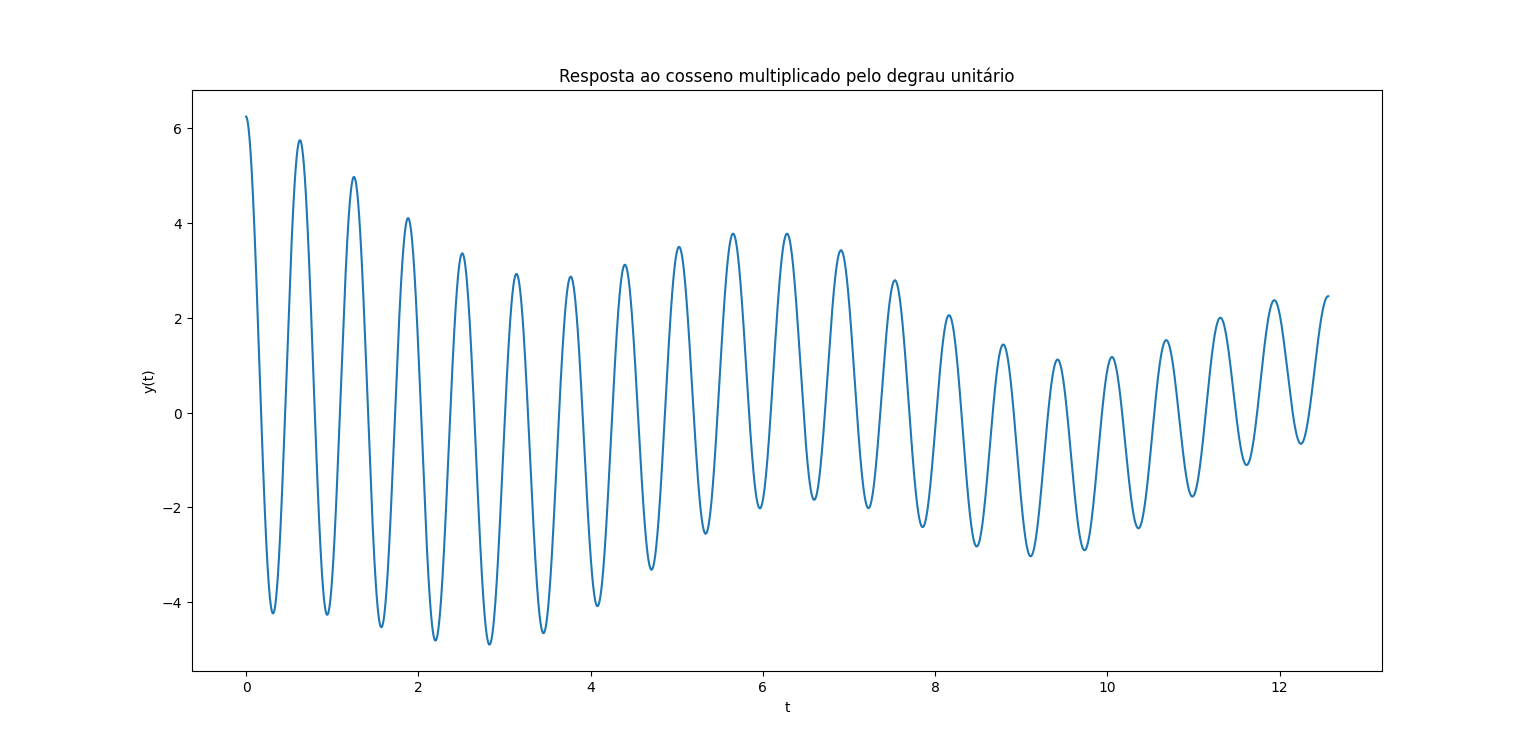
\includegraphics[scale=0.45]{Figure_1.png}
    \centering
\end{figure}

Solução analítica:

\begin{align*}
    y(t) = |H(j)| \cdot cos(t + \angle H(j)) = \frac{100}{16} \frac{\sqrt{(16-1^2)^2}}{\sqrt{0.04 + (100 - 1^2)^2}} \cdot cos(t + arctan(0/(16 - 1^2)) - arctan(0.2/(100 - 1^2))) = \\
    = \frac{100}{16} \frac{15}{\sqrt{0.04 + 99^2}} \cdot cos(t + 0 - arctan(0.2/99)) = \frac{100}{16} \frac{15}{99.000202} \cdot cos(t + 0.00202) = 0.946968 \cdot cos(t + 0.00202)
\end{align*}

2. Foi considerado uma entrada $u(t) = cos(4 t) 1(t)$ (frequência de zero). Foi obtido a resposta $y(t)$ por simulação numérica utilizando Python
e as bibliotecas NumPy, Matplotlib e Control.

3. Foi considerado uma entrada $u(t) = cos(10 t) 1(t)$ (frequência de zero). Foi obtido a resposta $y(t)$ por simulação numérica utilizando Python
e as bibliotecas NumPy, Matplotlib e Control.

4. Foi considerado uma entrada $u(t) = cos(100 t) 1(t)$ (frequência de zero). Foi obtido a resposta $y(t)$ por simulação numérica utilizando Python
e as bibliotecas NumPy, Matplotlib e Control.

Conclusão:

\end{document}